% Five real values of L(sigma, chi_{-4}) = sum_k ( (4k+1)^{-sigma} - (4k+3)^{-sigma} ).
% Rounded to three decimals from 0.6677, 0.7854, 0.8645, 0.9160, 0.9689.
% The value at sigma = 1 is pi/4. The vertical scale starts at 0.60.
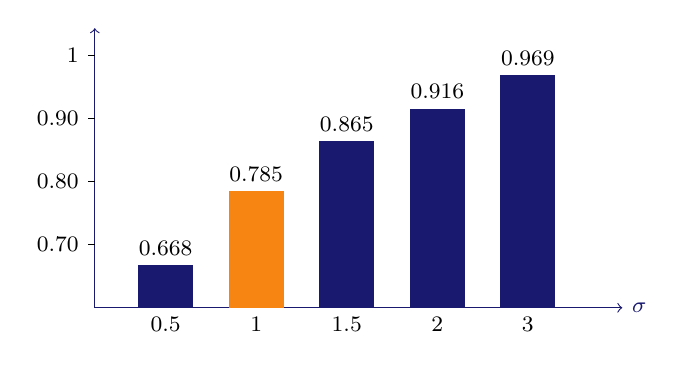
\begin{tikzpicture}[every node/.style={font=\footnotesize}]
  \draw[->,MidnightBlue] (0,0)--(6.7,0) node[right] {$\sigma$};
  \draw[->,MidnightBlue] (0,0)--(0,3.55);
  \draw (0,0.80)--(-0.08,0.80) node[left] {$0.70$};
  \draw (0,1.60)--(-0.08,1.60) node[left] {$0.80$};
  \draw (0,2.40)--(-0.08,2.40) node[left] {$0.90$};
  \draw (0,3.20)--(-0.08,3.20) node[left] {$1$};
  \fill[MidnightBlue] (0.55,0) rectangle (1.25,0.544);
  \fill[BurntOrange] (1.70,0) rectangle (2.40,1.480);
  \fill[MidnightBlue] (2.85,0) rectangle (3.55,2.120);
  \fill[MidnightBlue] (4.00,0) rectangle (4.70,2.528);
  \fill[MidnightBlue] (5.15,0) rectangle (5.85,2.952);
  \node[above] at (0.90,0.544) {$0.668$};
  \node[above] at (2.05,1.480) {$0.785$};
  \node[above] at (3.20,2.120) {$0.865$};
  \node[above] at (4.35,2.528) {$0.916$};
  \node[above] at (5.50,2.952) {$0.969$};
  \node[below] at (0.90,0) {$0.5$};
  \node[below] at (2.05,0) {$1$};
  \node[below] at (3.20,0) {$1.5$};
  \node[below] at (4.35,0) {$2$};
  \node[below] at (5.50,0) {$3$};
\end{tikzpicture}
